    \section{Introduction}
    
    This class and the sequel are concerned with covering the mathematics of thermodynamics, electromagnetism, and quantum mechanics. Of course, the mathematics supplied here is not limited to these fields, but it is hopefully presented in a way to align with those subjects.  At the heart of chemistry are the interactions in and between atoms and molecules. On the small scale, their interactions and structures are well understood via experiment and quantum theory. Zoom out a bit and electromagnetic effects take over. Zoom out further and we find that ensembles of large amounts of chemicals behave due to thermodynamic laws.  
    
    All of scientific theory is verified by experiment, but the theory itself is based in mathematics. A working scientist tends to lean towards either theorist or experimentalist, but one should be knowledgeable in both respects.  Think of mathematical theory as providing you with another form of analysis.  Mathematical knowledge will undoubtedly help you in your future scientific endeavors.  At the very least, it is an exercise in how to approach problems in a logical way.
    
    Take this course as a first dive into many new areas of math.  There will \emph{immediately} be a wealth of new terms and methods presented to you.  Learning what these are takes effort.  Even keeping terminology correct or what type of object (scalar, vector, matrix, function, etc.) something is can be confusing! Keep your mind open to questions.  Try not to fear math and it will work with you. Keep your head up and do not feel discouraged when the material feels tough.  It is tough for everyone.  Eventually you will improve your understanding. After this course and the sequel, you can look back at everything you have learned and smile!
    
    
    \section{How to read this text}
    
    What good is a textbook if you don't enjoy reading it? Or worse, what if you can't follow the material? Reading textbooks or scientific texts can be challenging, but you should think of it as another step in your career of learning!\\
    
\noindent    To get the most out of this textbook I suggest the following:
    \begin{enumerate}
        \item \emph{Pre-read}. Read through the relevant section once and try to see what the main point is.  Don't fuss over details! Go for big picture here. Maybe write down questions that come to you.
        \item \emph{Re-read}. Read the relevant section again. Yes, I am asking for you to do this twice! This time, go slower. Go through with a fine tooth comb and make sure you can make as much sense of the material as you can.  See if all the logic is true.  If there are exercises, attempt them.  Write down questions and bring them to class, office hours, or to a tutor.
        \item \emph{Review}. Come to class, office hours, or meet with other students/colleagues/tutors to go over the questions you have. As this says here, class should be more of a review than a first pass through. Having questions is great! It means learning is soon to follow. 
        \item \emph{Practice}. Do the homework and work through other exercises present in the text. This is the start to mastering a subject.  You may feel that you have gotten the material down but you can't \emph{know} that until you try.  Give the homeworks a try without notes or the text until you feel you need it! This aids in ability to recall.
        \item \emph{Correct}. None of us are perfect. Chances are that you may still miss something on an exercise or problem that you were sure that you had right.  Realize the mistake and integrate the new knowledge.  Sometimes this takes a bit of un-learning.  That can be tough, so be patient and forgiving with yourself.
        \item \emph{Reference}. There will be times where you will need to revisit some previous material.  Use this text as a reference for our class.  The more times you see something, the more it will stick.
    \end{enumerate}
    
    Sometimes there will be information stored away in problems, exercises, questions, answers, or remarks that is not otherwise explained in the text.  This is done when a bit of information is better discovered by the reader as opposed to being given away.  These problems will typically be labeled with an asterisk to denote their importance. I choose to use the following conventions.
    \begin{itemize}
        \item \emph{Problems}. Not assigned to be turned in, but should be done to check your knowledge once you have spent time with a portion of the text.  Problems will come after sections or subsections and important problems are marked with an asterisk.
        \item \emph{Exercises}. Exercises come within the body of a section or subsection. These should be, at the very least, read along with the other material to see what can be asked. In general, these are not meant to take too long. They should mostly check your current understanding. Think of them as passage to the next material.
        \item \emph{Questions}. Questions are put there for you to think about.  Almost always the questions will come along with an answer. Though you have an answer, you should work to understand \emph{why} it is the answer and if there is any more to be said.
        \item \emph{Answers}. Given to most questions. Think about these and make sure they make sense to you.
        \item \emph{Remarks}. These have nuggets of information that serve as a reminder or notify the reader about some subtleties. Note what these remarks mention and be sure to keep them in mind.
    \end{itemize}
    
    \subsection{Mathematical language}
    
    \subsubsection{Mathematical symbols}

    Here is a list of symbols you will find in our class (if more come, I will update this list):

    \begin{itemize}
        \item $\R$, The set of \emph{real numbers}.
        \item $\in$, ``Is a member of." (i.e. $\sqrt{2}\in \R$ can be read as, ``The square root of 2 is a member of the real numbers."
        \item $\neq$, \underline{Not} equal to.
        \item $\approx$, ``Approximately equal to."
        \item $\coloneqq$, We are defining something, i.e., $\frac{df}{dx}\coloneqq \lim_{h\to 0}\frac{f(x+h)-f(x)}{h}$.
        \item $\implies$, "Implies."
        \item $\iff$, "If and only if."
        \item $\therefore~$, "Therefore."
        \item $\infty$, Infinity.  \emph{Note: Infinity is \underline{not} a number!}
        \item $\delta$, A change. (i.e. $\delta x$ represents a change in the variable $x$).
        \item $\vecv$, a boldfaced character with an arrow will represent a vector.
        \item $(x_1,x_2,\dots,x_n)$, represent a (row) vector with $n$ components.
        \item $\begin{pmatrix} x_1\\ x_2\\ \vdots \\ x_n\end{pmatrix}$, a vector with $n$ components.
    \end{itemize}
    
    \subsubsection{Mathematical presentation}
    
    I have provided you with some ideas on how to read this text which tend to be good practice in general.  But, this is a mathematics text, how is it different? Well, mathematics tends to be presented in a specific way and it can come across as being utterly devoid of inspiration.  In truth, mathematics is discovered almost entirely backwards from how a text is written.  It's just the truth.
    
    Like other mathematical texts, we will often motivate a topic and define some terms that seem to be helpful along the way.  It's sometimes easiest to add new terms to a dictionary when they are often used.  We just call this a \emph{definition}. See for example, Definition \ref{df:invertible_functions}. Definitions will be placed in CSU-themed green boxes.
    
    Definitions are tautologically true since we have defined the very thing we would like.  However, we sometimes wish to show that what we have defined plays nicely together and gives us some new useful information.  These can come in many forms!  We have \emph{theorems}, \emph{propositions}, \emph{lemmas}, and \emph{corollaries}; Each with its own specific meaning.  All of these results will be placed in CSU-themed gold boxes as they are representing new information. Let's briefly say what each is.
    
    \begin{itemize}
        \item \emph{Theorem}. An important logical result that needs proof to be accepted.  Proof comes from logic that we previously develop.  A very useful example is the Pythagorean theorem. 
        \item \emph{Proposition}. A smaller independent result, but important nonetheless.
        \item \emph{Lemma}. A smaller result that tends to be working towards a larger one.  Many times, a theorem is proved by using multiple lemmas beforehand.  
        \item \emph{Corollary}. A result that follows fairly easily from a lemma or theorem.  Sometimes it's extra emphasis on using a very general theorem on something more specific, so it is literally not saying anything new but rather pointing the reader to this important consequence.
    \end{itemize}
    
    In this journey of mathematics we will come across each one.  The important thing for the reader is to understand the logic along the way.  Do you need to prove theorems? No, I will do that for you. More often than not, I will even omit proofs unless they are strategically enlightening.  However, one should always be suspicious if some logic seems incorrect. I promise you, there are no lies in this text, but it doesn't mean things are obvious!
    
    
    \section{Review}
    The prerequisite classes for this course are Math 155, Math 159, or Math 160.  Moreover, there is a requirement that the following topics are understood.  To check your understanding, work through all the listed problems in this review section. I repeat! Work through each problem in the review! If you can work through each problem and, better yet, understand each step you take through a solution, then you are well on your way to learning new material in this course.
    
    This course will require the following:
    \begin{enumerate}[1.]
        \item Computation.
        \item Algebra.
        \item Geometry.
        \item Trigonometry.
        \item Functions.
        \item Calculus.
    \end{enumerate}
    
    \noindent Below in each respective subsection are notes and example problems.  
    
    \subsection{Computation}
    
    What is computation? Computation is what we have drilled into our heads at a young age.  It's how many of us view mathematics up until we explore areas such as algebra.  Given an expression, how can we interpret it?  With this, we also need an agreed upon language.
    
    Typically we mean to output a real (or possibly complex) number from an expression.\footnote{Really we just need outputs we agree upon. The numbers I mentioned are common but there's no inherent reason that those two number systems are what your expression calls for!} This number tells us what an expression means. For example, the expression is about making some type of measurement. In scientific fields, that is common.
    
    \subsubsection{PEMDAS}
    
    PEMDAS, or 
    \[
    \textrm{Parentheses $\veryshortarrow$ Exponents $\veryshortarrow$ Multiplication $\veryshortarrow$ Division $\veryshortarrow$ Division $\veryshortarrow$ Addition $\veryshortarrow$ Subtraction},
    \]
    gives the standard order of operations.  This is simply a choice us humans have agreed on and made calculators or computer programming languages follow.  Good for avoiding arguments, probably.
    
    The reason I note this here is so that we can pay attention to properly computing expressions.  Often times students will find expressions such as
    \[
    -2^2 \qquad \textrm{and} \qquad (-2)^2
    \]
    to be equal. If you found them equal, can you see how they differ?
    
    Be cognisant of what the expression is \emph{really} telling you to do.  Use calculators or online tools like Wolfram Alpha as tools to check your answers. Often you will not have have a calculator available, so practicing without one is ideal.
    
    \subsubsection{Logarithms and exponents}
    
    Logarithms and exponents are extremely important classes of functions as well as tools.  Logarithms originally assisted in helping mathematicians do large computations as they can turn multiplication into addition which is arithmetically less challenging.  Both show up in nature quite often.  Let us revisit the necessary rules we must know about these functions.
    
    For the following table, $\log$ represents a logarithm of any base.  A base is only specified when needed. Think about which rules are redundant, if any!
    \begin{table}[H]
        \centering
        \renewcommand{\arraystretch}{1.5}
        \begin{tabular}{c|c|c}
            Rule & Logarithms & Exponents\\
            \hline
            Identity & $\log(1)=0$ & $a^0=1$\\
            \hline
            Inverse & $\log_a\left(a^x\right)=x$ & $a^{\log_a(x)}=x$\\
            \hline
            Multiplication & $\log(ab)=\log(a)+\log(b)$ & $a^x a^y=a^{x+y}$ \\
            \hline
            Division & $\log\left(\frac{a}{b}\right)=\log(a)-\log(b)$ & $\frac{a^x}{a^y}=a^{x-y}$\\
            \hline
            Power & $\log(a^p)=p\log(a)$ & $\left(a^x\right)^p = a^{px}$
        \end{tabular}
        \label{tab:log_exp_rules}
    \end{table}
    \emph{Challenge}: Can you derive these rules based on what each function's definition is? That is, remember that
    \[
    a^p = \underbrace{aa\cdots a}_{p \textrm{~times}}
    \]
    \footnote{If $p$ is not a positive integer, this is a bit harder to understand. Pretend that it is for this case.}and
    \[
    b^x = a \quad \textrm{means that} \quad \log_b(a)=x.
    \]
    If you don't try this, that's okay.  One mathematical exercise is to re-derive knowledge for yourself. Many people find it helps the learning process immensely!
    
    Lastly, remember what the magnitude of different powers tell us.  That is, I want you to be comfortable making the following identifications.
    
    \begin{align*}
        a\cdot a &= a^2,\\
        \sqrt{a} &= a^{1/2},\\
        \sqrt[p]{a} &= a^{1/p},\\
        a^{-1} &= \frac{1}{a},\\
        a^{-p} &= \frac{1}{a^p}.
    \end{align*}
    
    Armed with your previous knowledge and the above information, work on the problems below.
    
    \subsubsection{Problems}
    
    \begin{problem}
    Evaluate the following.
    \begin{enumerate}[(a)]
        \item $-3^2-2(3+2^2)$;
        \item $(-3)^2-2(3+2)^2$;
        \item $\frac{2-(-3)^2}{2^{(3-2)^2}}$.
    \end{enumerate}
    \end{problem}
    
    \begin{problem}
    Write the following as a simplified fraction:
    \[
    \frac{1}{2}-\frac{3}{5}.
    \]
    \end{problem}
    
    \begin{problem}
    Rewrite the following in an equivalent way using log and exponent rules. If no rules apply, say so.
    \begin{enumerate}[(a)]
        \item $\ln(2a)$;
        \item $\ln(2+a)$;
        \item $\ln(2^a)$;
        \item $\log_{10}(a^2)$;
        \item $\log_2(2^a)$.
    \end{enumerate}
    \end{problem}
    
    \begin{problem*}
    Recall that we can convert between different bases of logarithms. For example,
    \[
    \log_a(x)=\frac{\log_b(x)}{\log_b(a)}.
    \]
    Convert the following logarithms to the \emph{natural logarithm} (logarithm with base $e$) and evaluate the expression when possible.
    \begin{enumerate}[(a)]
        \item $\log_2(2)$;
        \item $\log_2(8)$;
        \item $\log_8(2)$;
        \item $\log_{10}(e)$;
        \item $\log_3(1)$;
        \item $\log_5(0)$.
    \end{enumerate}
    If an expression can't be evaluated, can you explain why?
    \end{problem*}
    
    \begin{remark}
    The name ``natural logarithm" will make more and more sense as we see how natural Euler's Number $e$ is.
    \end{remark}
    
    \begin{problem*}
    We can also convert between different bases for exponentials. Really, we just like to do this to convert to the exponential with Euler's number $e$. We have that
    \[
    b^x=e^{\ln(b)x}.
    \]
    Can you show this using the rules above? Convert the following to their natural exponential ($e^\textrm{something}$) counterpart or convert to the form $b^x$.
    \begin{enumerate}[(a)]
        \item $3^x$;
        \item $e^{\ln(2)x}$.
    \end{enumerate}
    \end{problem*}
    
    \subsection{Algebra}
    
    What is algebra? Algebra is Arabic for ``reunion of broken parts." It is a large and pervasive field of mathematics concerned with structure.  There are many different flavors as well.  Abstract algebra, linear algebra, and operator algebra are just a few examples. We will learn some of each of the named fields as we progress through the Math 271 and 272 courses.
    
    At this point, we treat algebra as manipulation of equations.  What one does to one side of an equation must do to the other in order to keep from changing the result or truth.  We are all familiar with this concept.  Clearly if 
    \[
    x=5
    \]
    and I only add $2$ to the right side,
    \[
    x=5+2=7,
    \]
    then our knowledge about $x$ has changed.  Albeit a simple example, this is \emph{exactly} what happens when we make algebra mistakes in our work.  Believe me, \emph{all} of us make algebra mistakes. 
    
    Practice with the problems below to review your understanding of algebra. They are given in no particular order.  Algebra is unbelievably fundamental in our pursuit of mathematical knowledge. We must make sure to have a strong foundation! 
    
    \subsubsection{Problems}
    
    \begin{problem}
    Solve the equation for $p$:
    \[
    3p-(5-2p)=2(p-3).
    \]
    \end{problem}
    
    \begin{problem}
    Solve the equation for $x$:
    \[
    12<\frac{9-x}{3}.
    \]
    \end{problem}
    
    \begin{problem}
    Which number(s) $x$ are in the interval $[2,6)$ and satisfy $x<4$?
    \end{problem}
    
    \begin{problem}
    Simplify the following.
    \[
    \frac{a^3b^4}{(ab)^2}=?
    \]
    What can we say if $a$ or $b$ is equal to zero?
    \end{problem}
    
    \begin{problem}
    Show that the following equalities are true using the rules given on exponents, fractional, and negative powers.
    \begin{enumerate}[(a)]
        \item $\displaystyle{\sqrt{x^2+x^2y^2}=x\sqrt{1+y^2}}$
        \item $\displaystyle{\frac{x^2+y^2}{x}=x+\frac{y^2}{x}}$
    \end{enumerate}
    \end{problem}
    
    
    \subsection{Geometry}
    
    What is geometry? Loosely speaking, geometry is the study of shape of space.  Geometry is concerned with distances, angles, size, and shape.  Many tools from more advanced geometry are distilled into a form that we will use throughout the time in Math 271 and Math 272.  At times, we will explore some of these concepts in a more advanced way (see linear algebra and multivariate calculus).
    
    For an introduction, knowing planar and spatial geometry is helpful.  One should be familiar with calculating areas and volumes as well as lengths and angles. The most important shapes to recognize will be circles and triangles as they satisfy some nice symmetries or properties.  We can use these two shapes along with some trigonometry to make geometrical inference.
    
    Here are some common volumes that may show up in Math 271 or the sequel, Math 272.
    
    \begin{figure}[H]
        \centering
        \includegraphics[width=.8\textwidth]{Figures_Part_1/volumes.png}
        \label{fig:volumes}
    \end{figure}
    
    % \subsubsection{Problems}
    
    
    % \begin{problem}
    % Compute the area of the following
    %     \begin{tikzpicture}
    %     \centering
    %     \draw[line width=1pt](0,0)--(3,1);
    %     \draw[line width=1pt](0,0)--(0,2);
    %     \draw[line width=1pt](0,2)--(3,1);
    %     \end{tikzpicture}
    % \end{problem}
    % areas, volumes, circles, triangles
    
    \subsection{Trigonometry}
    
    What is trigonometry? Think of trigonometry as the mathematics behind analyzing planar triangles and circles.  This comes down to using the well known trigonometric functions $\cos$, $\sin$, $\tan$, $\sec$, $\csc$, $\cot$. Of course, we often times care about the (pseudo) inverse functions of these as well. 
    
    One of the most important results in trigonometry is the Pythagorean Theorem. We will use it all throughout this course in one way or another.  Let us state it below. 
    
    \begin{thm}{Pythagorean Theorem}{pythag}
    Let $\triangle$ be a right triangle with side lengths $a$, $b$, and $c$ shown below.
    \begin{figure}[H]
        \centering
        \includegraphics[width=.3\textwidth]{Figures_Part_1/right_triangle.png}
    \end{figure}
    Then we have that $c^2=a^2+b^2$.
    \end{thm}
    
    % \textcolor{blue}{Degrees and radians, cosines, sines of angles and what they represent. Why a circle has $2\pi$ radians. We can compute distances in the plane using pythagorean}
    
    % \subsubsection{Problems}
    
    
    \subsection{Functions}
    
    What are functions? Functions are machines that give a single output for a given input. This is something you may have heard called the ``vertical line test" when you were looking at graphs of real values functions. But, Beware! That doesn't mean that each single input corresponds to a single output. Many inputs can have the same output. More on this later.
    
    We often use functions to represent relationships or measurements.  Analyzing functions is of utmost importance when we wish to gain insight from them.  For us, functions will typically be thought of as some physical variable (think temperature, velocity, or probability). We'll also learn that functions can be solutions to certain kinds of expressions called \emph{differential equations}.  
    
    There is a lot of terminology and notation surrounding functions. Let us cover the necessary details. 
    
    \subsubsection{Notation and terminology}
    
    We typically represent a function (of a single variable) by $f(x)$ and say ``$f$ of $x$." Of course, the function $f$ and input $x$ can be represented by any symbols you'd like.  Maybe you want to have a function $\smiley(\uparrow)$ which we would say ``smiley of up-arrow." We tend to stick with notation others use to stay a bit more sane.
    
    Mathematicians really like to specify a function by writing
    \[
    f\colon D \to C
    \]
    which can be read as ``$f$ inputs variables from the set $D$ and outputs an element from the set $C$." Here, $D$ is the \emph{domain} and $C$ is the \emph{codomain}. This notation is handy when we deal with functions that have different inputs and outputs than we have handled before. So, mathematicians shouldn't be the only ones to like this notation!
    
    So far, what I have provided above does not specify what the function actually does.  For this, we usually provide an expression like
    \[
    f(x)=x^2
    \]
    which tells us to square each input to get the output or we can specify the function to take certain values when given a certain input, i.e.,
    \[
    f(2)=3.
    \]
    
    
    \subsubsection{Domain, codomain, and range}
    
    The domain and range of a function are always specified. However, sometimes the specification is understood and we don't list it.  The \boldgreen{domain}\index{domain} $D$ of a function is the set of all input values.  The \boldgreen{codomain}\index{codomain} $C$ of a function is the set that output values can live in.  \emph{Note, \underline{not} all elements in the codomain are necessarily output by the function!} The \boldgreen{range}\index{range} $R$ of a function is the set of all output values.  
    
    \begin{question}
    Is the codomain $C$ a larger, smaller, or same size set as the range $R$?
    \end{question}
    
    \begin{answer}
    This was a bit of a trick question.  The codomain is \emph{at least as big} as the range as it contains all the output values the function \emph{could} hit.  The range may have the same exact elements of the codomain and the range could be smaller than the codomain.
    \end{answer}
    
    \begin{ex}{Codomain and Range for Finite Sets}{codomain_range}
    \begin{enumerate}[(i)]
        \item Let $f$ be a function with domain $D=\{1,2,3\}$ (i.e., $D$ is the set of numbers one, two, and three) and codomain $C=\{1,2,3,4\}$. We can say that 
    \[
    f\colon D \to C
    \]
    and we completely define $f$ by choosing an output for each input. We'll take
    \begin{align*}
        f(1)&=1;\\
        f(2)&=1;\\
        f(3)&=4.
    \end{align*}
    As stated, the codomain is the set $\{1,2,3,4\}$, but what is the range $R$? Since we have specified an output for every input, we can just look at the list of outputs which is
    \[
    f(1)=1,~f(2)=1,~f(3)=4,
    \]
    and so the range $R=\{1,4\}$.  Notice that the range is strictly smaller than the codomain. Also, this function does \underline{not} output a unique value for each given input.
    
        \item Let $g$ be a function on the same domain and codomain as in (i). That is,
        \[
        g\colon D \to C.
        \]
        Let us define $g$ as we did with $f$ by specifying the output for each input.
        \begin{align*}
            g(1)&=2;\\
            g(2)&=3;\\
            g(3)&=4.
        \end{align*}
        Again, one should check that the range is smaller than the codomain. Also, check whether this function has a unique output for each input. 
    \end{enumerate}
    \end{ex}
    
    \begin{question}~
    \begin{itemize}
        \item Given an output value for the function $g$ above, can one determine what the input value had to be?
        \item How about for $f$?
        \item What is the difference between these two? 
    \end{itemize}
    \end{question}
    
    \begin{answer}~
        \begin{itemize}
            \item Yes we can. We call this association the \emph{inverse function}.
            \item No, not quite.  For example, what input gives us the output value of 1?
            \item $g$ is a \emph{one-to-one} function. It has a unique input value for each output value. $f$ is \underline{not} one-to-one.  Inverting $f$ is not really possible.
        \end{itemize}
    \end{answer}
    
    \begin{ex}{Codomain and Range for $\R$-Functions}{codomain_range_real}
        Let us work with functions we are likely more familiar with.  
        \begin{enumerate}[(i)]
            \item Let $f$ be a real valued function of one real variable. That is, 
            \[
            f\colon \R \to \R.
            \]
            We understand this as $f$ takes in a real value and outputs a real value as well.  This is just some extra notation and verbage for something we already understand!
            
            Since $\R$ is infinite, us humans can't really specify an output value for every input.  Instead, we provide an association.  Let's define $f$ by saying what $f$ \emph{does} to some input value.  Let
            \[
            f(x)=x^2.
            \]
            Now, the codomain for $f$ is all the real numbers $\R$ but the range $R$ for $f$ is smaller.  Since we are squaring the input to get the output, the range of $f$ is $R=[0,\infty)$.  We can't achieve negative values! Notice also that $f$ is not one-to-one.
            
            \item Let's define a new function $g\colon \R \to \R$ by letting
            \[
            g(x)=x^3.
            \]
            The range in this case is $\R$ and $g$ is one-to-one. You should verify these facts.
        \end{enumerate}
    \end{ex}
    
    
    \subsubsection{Composition}
    
    If we have functions $f$ and $g$, we may want to look at how we can string the two together.  First, we should say what we mean by this and determine when it is even possible to do so.  Let's say that we have
    \begin{align*}
        f\colon D_1 &\to C_1,\\
        g\colon D_2 &\to C_2,
    \end{align*}
    and the range for $f$ and $g$ is $R_1$ and $R_2$ respectively.  We want to consider the composition of functions
    \begin{align*}
        (f\circ g)(x) &= f(g(x)),\\
        (g\circ f)(x) &= g(f(x)).
    \end{align*}
    
    \begin{question}
    When are we allowed to \emph{compose} the function $f$ with $g$ as $f\circ g$? How about as $g\circ f$?
    \end{question}
    
    \begin{answer}
    Let's think of this in an analogy.  If $f$ converts from Spanish to English and $g$ converts from German to Spanish, how can we string the two translators together to convert from German to English?  
    
    Think of $x$ as a word in German.  If we then look at $g$ translating $x$,
    \[
    g(x)=y,
    \]
    then $y$ is now some word in Spanish.  Now, $f$ is happy to translate this word right on over to English by
    \[
    f(y)=z,
    \]
    where $z$ is our desired English word.  So, we have really done the following:
    \[
    (f\circ g)(x)=f(g(x))=f(y)=z.
    \]
    
    Now, in terms of functions on sets of numbers, we want to think like in this above analogy.  The output of one function $g$ better agree with the input $f$ knows how to handle.  More below.
    \end{answer}
    
    If we have that the range $R_1$ is in the domain $D_2$, then we can have the composite function
    \[
    g\circ f,
    \]
    and
    \[
    g\circ f \colon D_1 \to C_2.
    \]
    This may be fairly abstract and confusing.  Don't worry too much! We'll keep seeing the point of this way of thinking over time. Let this knowledge grow slowly over time.
    
    \begin{exercise}
    Repeat the above if we have that the range $R_2$ is in the domain $D_1$.
    \end{exercise}
    
    \subsubsection{Inverse functions}
    
    We have all seen \emph{inverse functions}, but let us re-familiarize ourselves with them just a bit while also giving a preview of the style of text to come.
    
    \begin{df}{Invertible Functions}{invertible_functions}
    Let $f\colon D \to C$ be a function. We say that $f$ is \boldgreen{invertible}\index{invertible} if for any value $y\in C$ there is a corresponding unique input $x\in D$.  That is to say, if we have $f(x)=y$ then the inverse function, $f^{-1}$, satisfies
    \[
    f^{-1}(y)=x.
    \]
    The inverse function \emph{undoes} the original function. So we have that
    \[
    (f^{-1}\circ f)(x)=x
    \]
    and
    \[
    (f\circ f^{-1})(y)=y.
    \]
    for every $x$ and every $y$.
    \end{df}
    
    \begin{remark}
    There's more subtleties here than meets the eye.  I'm going to avoid them for now.  But if you'd like more to think about, consider the composition function
    \[
    f\circ f^{-1}.
    \]
    What will we have to know about domains, ranges, or codomains? Careful.
    \end{remark}
    
    Alluded to earlier was the idea of a function that is one-to-one. Let's define that here and now.
    \begin{df}{One-to-one Function}{one_to_one}
    Let $f\colon D \to C$ be a function. We say that $f$ is \boldgreen{one-to-one} if for each output value $y$ there is a unique input value $x$.
    \end{df}
    \noindent Take a moment to soak this one in. Revisit Example \ref{ex:codomain_range} and Example \ref{ex:codomain_range_real}. Think of a few examples of functions that are and are \underline{not} one-to-one.
    
    Another important notion is that of a function whose range is equal to the codomain.  We made sure to see that there could be differences before, so let's define this notion.
    
    \begin{df}{Onto Function}{onto_fxn}
    Let $f\colon D \to C$ be a function with range $R$. If we have $R=C$, then $f$ is \boldgreen{onto}\index{onto}.
    \end{df}
    
    While we're at it, we may as well introduce a proposition. This is not a groundbreaking result as the definitions we have really play nicely together. 
    
    \begin{prop}{One-to-one and Onto Functions are Invertible}{one_to_one-invertible}
    \textit{If $f\colon D \to C$ is a one-to-one and onto function if and only if it is also invertible.}
    % \noindent \emph{Proof.} Suppose the $f$ is one-to-one, then we know that for each output $y$, there is a unique input $x$.  Thus, we can define an inverse function that, given the input $y$, assigns an output $x$. That is, we make $f^{-1}(y)=x$, which is indeed a function since for each input we have a unique output. Thus, $f$ is invertible.
    
    % For the converse, we suppose that $f$ is invertible and we have $f^{-1}$ as the inverse function.  Since $f^{-1}$ is a function, it must assign a unique output value for each input.  This means that $f$ must only assign a unique output for each unique input, or else this could not be trust. Hence, it follows that $f$ is one-to-one. \qed
    \end{prop}
    Right now, we're avoiding any proof.  This one isn't too bad, but I'll restate that proofs are not part of this course. Proofs take time to understand and it's challenging to develop the skills to write them properly!  That's why the mathematics majors at CSU take Math 235 as an introduction to mathematical reasoning.  It truly is a challenge in its own right.
    
    
    \subsubsection{Visualizing functions}
    When working with real valued functions of one real variable (again, $f\colon \R \to \R$), we often draw the \emph{graph} of the function in the plane.  The function knows nothing about how we like to look at it, and it's important to realize that this is merely a human adaptation.  We'll eventually learn \emph{exactly} what it is that we do when we graph a function, but give it time.  For the mean time, just revisit the idea yourself.
    
    \begin{ex}{Graphing a Function}{graphing_function}
    Let's consider the function $f\colon \R \to \R$ given by $f(x)=x^2$.  The the \boldgreen{graph}\index{graph} of $f$ is the set of points $(x,f(x))$ that we highlight in the $xy$-plane.  So, the graph for this $f$ follows.
    \begin{center}
    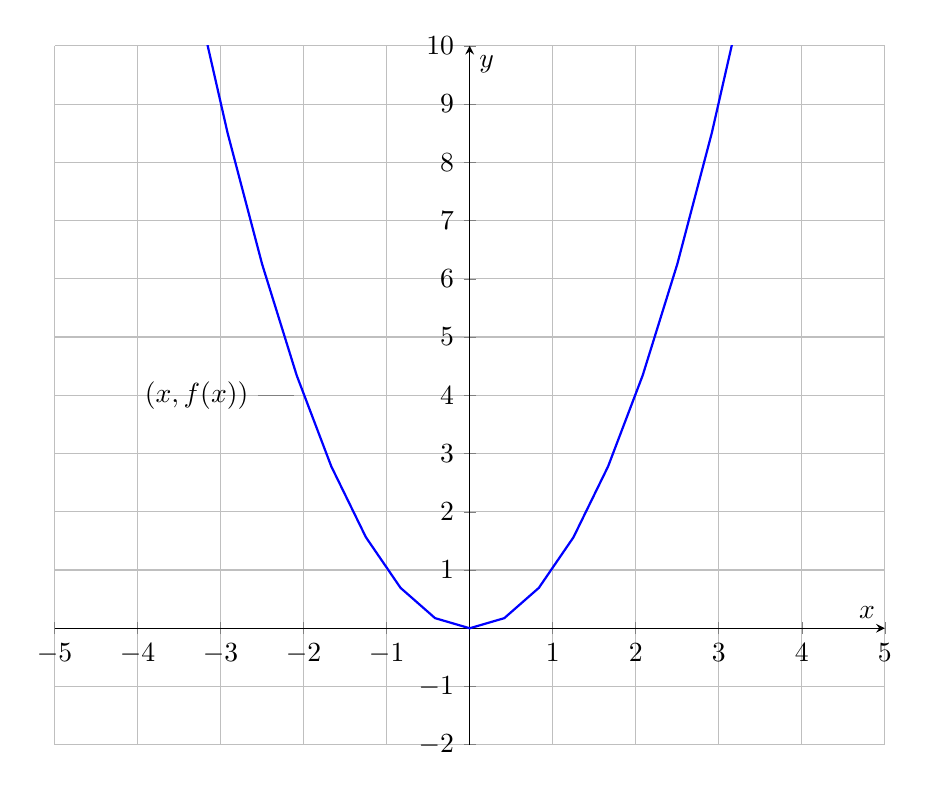
\begin{tikzpicture}[baseline]
    \begin{axis}[
    axis y line=center,
    axis x line=middle,
    %axis equal,
    grid=both,
    xmax=5,xmin=-5,
    ymin=-2,ymax=10,
    xlabel=$x$,ylabel=$y$,
    xtick={-10,...,10},
    ytick={-10,...,10},
    width=\textwidth,
    anchor=center,
    ]
    \addplot [mark=none, blue, thick]{x^2} ;
    \addplot [mark=none] coordinates {(-2,4)} node[pin=180:{$(x,f(x))$}]{};
    \end{axis}
    \end{tikzpicture}
    \end{center}
    \end{ex}
    
    Similar techniques for visualizing functions in higher dimensions will come. For now, just practice with functions of one real variable.
    
    \subsubsection{Problems}
    
    \begin{problem}
    Let $f(x)=x^2$. 
    \begin{enumerate}[(a)]
        \item Show that
        \[
        f(x+y)=x^2+2xy+y^2.
        \]
        \emph{Warning!} There is a common error made here. Do not fall victim to believing that
        \[
        f(x+y)=f(x)+f(y)
        \]
        for \underline{all} functions.  Functions that have this property are \emph{special}!
        \item Show that
        \[
        f(\lambda x)=\lambda^2x^2.
        \]
    \end{enumerate}
    \end{problem}
    
    \begin{problem}
    Let $g(r)=\frac{\hbar}{2}(r+r^2)$. Evaluate and simplify the following.
    \begin{enumerate}[(a)]
        \item $g(a+b)$;
        \item $g(\lambda a + x)$;
        \item $g(r^2)$.
    \end{enumerate}
    \end{problem}
    
    \begin{problem}
    Let $r(\smiley)=\frac{1}{\smiley^2}$. Evaluate and simplify the following.
    \begin{enumerate}[(a)]
        \item $\left[r(\smiley)\right]^2$;
        \item $r(-\smiley)$;
        \item $-r(\smiley)$.
        \item $r(\smiley)+r(2\smiley)$.
        \item $r(\smiley)+2r(\smiley)$.
        \item $r(\smiley^2)+r(2\smiley)+2r(\smiley)$.
    \end{enumerate}
    \end{problem}
    
    \begin{remark}
    Just remember, the function and variable letters are arbitrary. Pay attention on how to properly evaluate a function with a given input despite aesthetic differences.
    \end{remark}
    
    \begin{problem}
    Find the domain and range of $f(x)=\sqrt{9-x}$.
    \end{problem}
    
    \begin{problem}
    Find the domain and range of $h(t)=\sqrt[3]{2-x^2}$.
    \end{problem}
    
    \begin{problem}
    Let $f(x)=5x+1$ and $g(x)=x^2$.
    \begin{enumerate}[(a)]
        \item Write the composite function $(g\circ f)(x)$.
        \item Write the composite function $(f\circ g)(x)$.
    \end{enumerate}
    \end{problem}
    
    \begin{problem}
    Use the table to find $(f\circ g)(3)$
    \begin{center}
    \begin{tabular}{|c||c|c|c|c|c|c|}
        \hline
        $x$ & -2 & -1 & 0 & 1 & 2 & 3 \\
        \hline
        $f(x)$ & 0 & 6 & 4 & -1 & 3 & -2\\
        \hline
        $g(x)$ & 5 & 3 & 2 & 1 & -1 & 0\\
        \hline
    \end{tabular}
    \end{center}
    \end{problem}
    
    \begin{problem}
    State if the given functions are inverses of each other. Be sure to check both $(f\circ g)$ and $(g\circ f)$ to see that this is true.
    \begin{enumerate}[(a)]
        \item $\displaystyle{f(x)=4-\frac{3}{2}x}$ and $g(x)=\displaystyle{\frac{1}{2}x+\frac{3}{2}}$;
        \item $f(x)=11x-2$ and $\displaystyle{g(x)=\frac{x+2}{11}}$.
    \end{enumerate}
    \end{problem}
    
    \begin{problem}
    Find the inverse for the following functions. If one does not exist, explain why. If a domain isn't specified, assume that it is $\R$.
    \begin{enumerate}[(a)]
        \item $f(x)=x^3$.
        \item $g(x)=x^2$.
        \item $h(x)=\sqrt{x}$.
        \item $l(x)=8x+3$.
        \item $p(x)=\sqrt[3]{x}-3$.
    \end{enumerate}
    \end{problem}
    
    
    
    \subsection{Calculus}
    
    So far, all of us have studied the calculus of functions of one real variable.  It just so happens that the techniques developed there will generalize nicely to higher dimensional cases.  However, it will take some careful thought along the way.  What's the point anyway?
    
    Calculus is the study of rates of change of functions.  I like to think about it as the study of functions on the very small scale.  On the small scale, you found that functions look almost linear.  It's not hard to see this!  Take any function of your liking and zoom in on a specific region of this function. Keep zooming in and you'll notice that at some point the function looks like a line.  This idea allowed us to look at the \emph{derivatives} of functions as well as help us compute \emph{integrals} of functions!  It's extremely important.  It will also relate to a beautiful field of mathematics known as linear algebra. 
    
    Studying change is about all we ever do as scientists.  Even systems that \emph{don't} change over time can be thought of as just having no rate of change! As we turn knobs or mix chemicals we watch for change. We record this change and study the properties both before and after.  It is undoubtedly important for all of us to know a nice way to analyze changes of systems. This is captured elegantly by calculus.
    
    \subsubsection{Derivatives}
    \emph{Derivatives} were introduced to study change of functions.  First, we looked at average rates of change of functions over an interval.  Say we have a function $f\colon \R \to \R$ and we want to find its average rate of change from $x_0$ to $x_1$, then we would compute
    \[
    \frac{\Delta f}{\Delta x} = \frac{f(x_1)-f(x_0)}{x_1-x_0}.
    \]
    But, what if we make this interval very \emph{very} small?  We would then be looking at functions on this very small scale where, graphically, they look like lines. As the interval shrank to zero, or we took
    \[
    \lim_{x_1 \to x_0} \frac{f(x_1)-f(x_0)}{x_1-x_0},
    \]
    we arrive at an instantaneous rate of change.
    
    Recall that a \boldgreen{derivative}\index{derivative} is the instantaneous rate of change of a (single variable) function. We defined the derivative $f'$ of $f$ at the point $x$ to be
    \[
    f'(x)\coloneqq\lim_{\Delta x \to 0} \frac{f(x+\Delta x)-f(x)}{\Delta x}.
    \]
    Can you see how the the two limits given are the same? We also had the notation
    \[
    \frac{d}{dx}f(x)=f'(x),
    \]
    which is nice to use at times. It will be especially helpful in the future to use the latter (Leibniz) notation.  Recall also that we had a handful of derivative rules.  Keep these near and dear to your heart.
    
    
    %Consider using longtable here somehow
    \begin{table}[H]
        \centering
        \renewcommand{\arraystretch}{2.5}
        \begin{tabular}{c|c}
            Rule & Derivative\\
            \hline
            Sum & $\displaystyle{\frac{d}{dx}(f(x)+g(x))=f'(x)+g'(x)}$\\
            \hline
            Constant Multiple & $\displaystyle{\frac{d}{dx}(c f(x))=cf'(x)}$\\
            \hline
            Product & $\displaystyle{\frac{d}{dx}(f(x)g(x))=f'(x)g(x)+f(x)g'(x)}$\\
            \hline
            Quotient & $\displaystyle{\frac{d}{dx}(f(x)/g(x))}=\frac{f'(x)g(x)-f(x)g'(x)}{\left[g(x)\right]^2}$\\
            \hline
            Chain & $\displaystyle{\frac{d}{dx}f(g(x))=f'(g(x))g'(x)}$\\
            \hline
            Power & $\displaystyle{\frac{d}{dx}x^p=px^{p-1}}$\\
            \hline
            Log & $\displaystyle{\frac{d}{dx}\ln(x)=\frac{1}{x}}$\\
            \hline
            Exponential & $\displaystyle{\frac{d}{dx}e^x=e^x}$\\
            \hline
            Sine & $\displaystyle{\frac{d}{dx}\sin(x)=\cos(x)}$\\
            \hline
            Cosine & $\displaystyle{\frac{d}{dx}\cos(x)=-\sin(x)}$
        \end{tabular}
        \label{tab:der_rules}
    \end{table}
    These will be all the necessary rules to know moving forward.  This list is actually quite redundant. Can you see which you can find from others?
    
    
    \subsubsection{Integrals}
    \emph{Integration} is the other fundamental technique learned in an introductory calculus course.  The idea is to be able to add up function values over an interval. This helped to also develop the ability to find area under a curve.  There are a few things to note here.
    
    Remember that an \boldgreen{integral}\index{integral} can be in the form of \boldgreen{definite integrals}\index{integral!definite} or as \boldgreen{indefinite integrals}\index{integral!indefinite}. The former returns a number that tells one the \emph{net} area under the graph of function.  Indefinite integrals, on the other hand, return a function that we so joyfully refer to as the \boldgreen{anti-derivative}\index{anti-derivative}. 
    
    We have some integration rules as well, but it is a shorter list. For now.
    \begin{itemize}
        \item Sum rule: $\displaystyle{\int f + g dx=\int f dx + \int g dx}$.
        \item Constant multiple rule: $\displaystyle{\int cf dx = c \int f dx}$.
    \end{itemize}
    
    There is one important theorem that we all need to remember here and before we begin a new voyage.  That is the following.
    
    \begin{thm}{Fundamental Theorem(s) of Calculus}{ftc}
    Let $f\colon [a,b] \to \R$ be a differentiable function with derivative $f'$.  Then we have the following:
    \[
    \int_a^b f'(x)dx = f(b)-f(a).
    \]
    
    We can also say that 
    \[
    \int f'(x)dx = f(x)+c
    \]
    for some constant $c\in \R$ as well as
    \[
    \frac{d}{dx} \int f(x)dx = f(x).
    \]
    \end{thm}
    \noindent This theorem is very fundamental to the study of calculus, hence the name!
    
    One should be familiar with how to perform \boldgreen{integration by substitution}\index{integral!integration by substitution} or a \emph{$u$-substitution}. That is, given an integral of the form
    \[
    \int_a^b f(g(x))g'(x)dx
    \]
    one can make a substitution letting $u=g(x)$ and noting that $du=g'(x)dx$.  Of course, many integrals are not of this form, but surprisingly many are. Anyways, we find that with this substitution we have
    \[
    \int_a^b f(g(x))g'(x)dx= \int_{g(a)}^{g(b)}f(u)du.
    \]
    
    \begin{ex}{Integration by Substitution}{int_by_sub}
        Consider the definite integral
        \[
        \int_1^2 2x\sin\left(x^2\right)dx.
        \]
        Notice that the $2x$ looks like the derivative of the inside of $\sin\left(x^2\right)$.  So we let $u=x^2=g(x)$ and we have $du=2xdx$. Thus we have
        \begin{align*}
            \int_1^2 2x\sin\left( x^2\right)dx &= \int_1^4 \sin(u)du\\
            &= -\cos(4)+\cos(1).
        \end{align*}
    \end{ex}
    
    After this technique comes one that may not be seen in any prerequisite course for this class.  This new technique is known as \boldgreen{integration by parts}\index{integral!integration by parts}. Integration by parts is a combination of the derivative product rule and the fundamental theorem of calculus.  Given functions $u(x)$ and $v(x)$ we can write
    \[
    (uv)'=u'v+uv'.
    \]
    Then if we integrate both sides, we have
    \[
    \int_a^b (uv)'dx = \int_a^b u'vdx + \int_a^b uv'dx.
    \]
    Fundamental theorem of calculus gives us that
    \[
    \int_a^b (uv)'dx = u(b)v(b)-u(a)v(a)
    \]
    and thus
    \[
    \int_a^b u'vdx = u(b)v(b)-u(a)v(a)-\int_a^b uv'dx.
    \]
    Or, without bounds on the integral, we can write
    \[
    \int u'vdx = uv - \int uv'dx.
    \]
    I like to think of integration by parts as shifting the derivative from one function to another with a penalty term.  Above, we swap a derivative on $u$ to a derivative on $v$ but have to correct with the function $uv$.  This can all be derived in higher dimensions using Stokes' theorem. It's an excellent tool in the study of differential equations.
    
    \begin{ex}{Integration by Parts}{int_by_parts}
        Consider the indefinite integral
        \[
        \int xe^x dx.
        \]
        Now $x$ is a function that gets ``simpler" when we take a derivative since $\frac{d}{dt}x= 1$.  So we wish to pick $v=x$ so $v'=1$ and hence $u'=e^x$ and we then have $u=e^x$ as well.  Plugging this in, we find
        \begin{align*}
            \int xe^x dx = \int u'vdx &= uv - \int uv'dx\\
            &= xe^x-\int_e^xdx\\
            &= xe^x - e^x + c.
        \end{align*}
    \end{ex}
    
    \subsubsection{Problems}
    
    \begin{problem}
    Compute derivatives for the following functions.
    \begin{enumerate}[(a)]
        \item $f(x)=18x^3+2x^2$;
        \item $g(x)=\sqrt{x+5}$;
        \item $h(x)=\sqrt{\frac{1}{x}}$;
        \item $p(x)=\sqrt[5]{x^3+15x}$;
        \item $q(x)=\frac{1}{\sqrt[4]{2x}}$;
        \item $r(x)=\sqrt{x^2}$. \emph{Hint: You can't cancel the square root and the square as they are \underline{not} proper inverses! Is this function differentiable everywhere? Plot it if need be.}
    \end{enumerate}
    \end{problem}
    
    \begin{problem}
    Compute derivatives for the following functions.
    \begin{enumerate}[(a)]
        \item $f(x)=xe^x$;
        \item $g(x)=e^{2x}$;
        \item $h(x)=b^x$;
        \item $p(x)=(x^2+2x)\ln(x)$;
        \item $q(x)=\ln\left(\frac{1}{x}\right)$;
        \item $r(x)=x^x$. \emph{Hint: This is tough. Try taking a natural log of both sides before differentiating.}
    \end{enumerate}
    \end{problem}
    
    \begin{problem}
    Compute derivatives for the following functions.
    \begin{enumerate}[(a)]
        \item $f(x)=\tan(x)$;
        \item $g(x)=\sec(x)$;
        \item $h(x)=\csc(x)$;
        \item $p(x)=\cot(x)$;
        \item $q(x)=\tan(\sin(\cos(x)))$.
    \end{enumerate}
    \end{problem}
    
    \begin{problem}
    Compute the following.
    \begin{enumerate}[(a)]
        \item $\displaystyle{\frac{d}{dx}\left(15y+15x\right)}$;
        \item $\displaystyle{\frac{d}{dy}\left(15y+15x\right)}$;
        \item $\displaystyle{\frac{d}{dr}\left(15y+15x\right)}$;
        \item $\displaystyle{\frac{d}{dx}\left(5x^2y+32y^3+5xy^2\right)}$;
        \item $\displaystyle{\frac{d}{dy}\left(5x^2y+32y^3+5xy^2\right)}$.
    \end{enumerate}
    \end{problem}
    
    \begin{problem}
    Compute the following antiderivatives. \emph{Do not forget the $+c$!}
    \begin{enumerate}[(a)]
        \item $\displaystyle{\int 2xdx}$;
        \item $\displaystyle{\int \cos(x)dx}$;
        \item $\displaystyle{\int \sec^2(x)dx}$.
    \end{enumerate}
    \end{problem}
    
    \begin{problem}
    Compute the following integrals.
    \begin{enumerate}[(a)]
        \item $\displaystyle{\int_0^2 x^3 dx}$;
        \item $\displaystyle{\int_{-1}^1 \sin(x)dx}$;
        \item $\displaystyle{\int_{-1}^1 |x|dx}$.
    \end{enumerate}
    \end{problem}
    
    \begin{problem*}
    The following is the definition of the natural logarithm:
    \[
    \ln(x)\coloneqq\int_1^x \frac{1}{x}dx.
    \]
    \begin{enumerate}[(a)]
        \item Using the Fundamental Theorem of Calculus, show that
        \[
        \frac{d}{dx}\ln(x)=\frac{1}{x}.
        \]
        \item Show and explain why
        \[
        \ln(1)=0.
        \]
        \item Show and explain why $\ln(0)$ is undefined.
    \end{enumerate}
    \end{problem*}
    
    % \begin{problem}
    
    % \end{problem}
    
    

    

